	See \tabref{tab:10/7/1/6/inner},
	\figref{fig:10/7/1/6/Fig1}, \figref{fig:10/7/1/6/Fig2}.
	and 
	\figref{fig:10/7/1/6/Fig3}. 
In b), forming the collinearity matrix
\begin{align}
\myvec{\vec{B}-\vec{A} & \vec{C}-\vec{B}} 
=
		\myvec{6&-3\\-4&2} \xleftrightarrow{R_{2}\rightarrow R_{2}+\frac{2}{3}R_{1}}= \myvec{6&-3\\0&0}
\end{align}
which is a rank 1 matrix.  Hence, $\vec{A}, \vec{B}, \vec{C}$  are collinear.
\begin{figure}[H]
	\begin{center} 
	    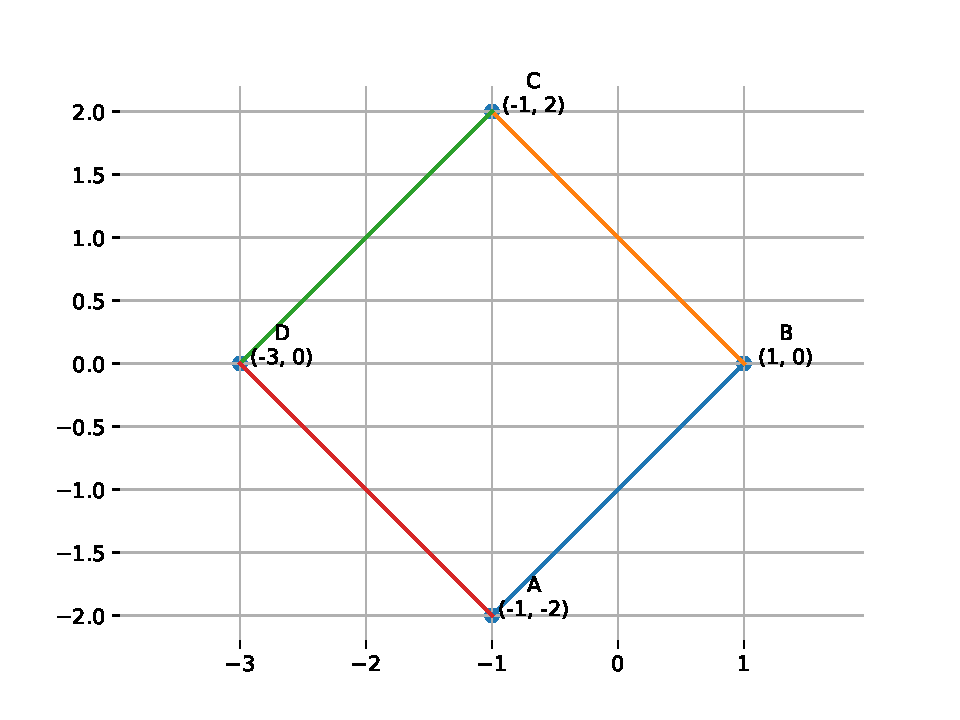
\includegraphics[width=0.75\columnwidth]{chapters/10/7/1/6/figs/fig1.pdf}
	\end{center}
\caption{}
\label{fig:10/7/1/6/Fig1}
\end{figure}
%
\begin{figure}[H]
	\begin{center} 
	    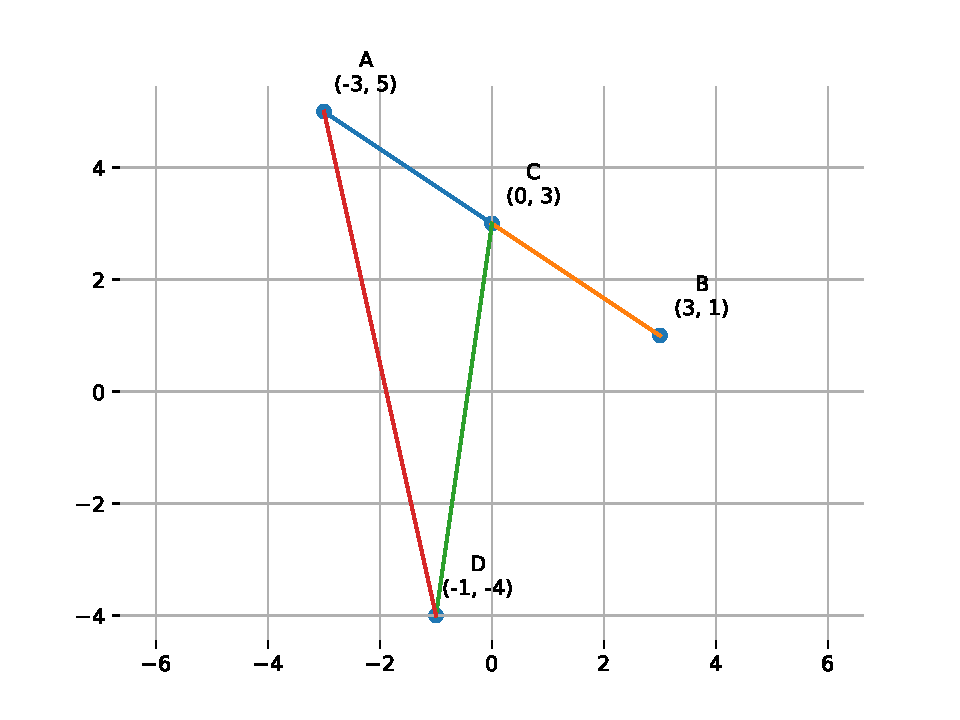
\includegraphics[width=0.75\columnwidth]{chapters/10/7/1/6/figs/fig2.pdf}
	\end{center}
\caption{}
\label{fig:10/7/1/6/Fig2}
\end{figure}
%	
\begin{figure}[H]
	\begin{center} 
	    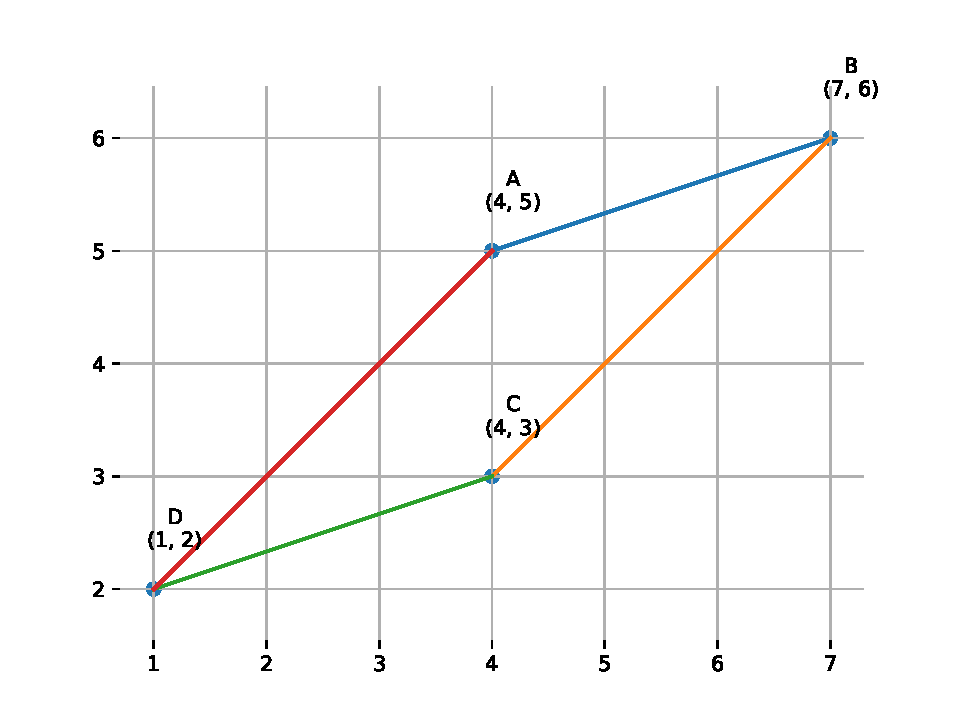
\includegraphics[width=0.75\columnwidth]{chapters/10/7/1/6/figs/fig3.pdf}
	\end{center}
\caption{}
\label{fig:10/7/1/6/Fig3}
\end{figure}
%
\begin{table}[H]
    \centering
%    \begin{tabular}{|c|c|c|c|c|}
	    \begin{tabularx}{\columnwidth}{|c|X|X|X|c|}
        \hline
		    &{\scriptsize $\vec{B}-\vec{A} = \vec{C}-\vec{D}$?} & {\tiny $(\vec{B}-\vec{A})^\top (\vec{C}-\vec{B}) =  0$?} & {\tiny $(\vec{C}-\vec{A})^\top (\vec{D}-\vec{B}) = 0$}& \textbf{Geometry}\\
        \hline
	    a)& Yes & Yes & Yes& Square \\
        \hline
	    b)& No & -&- & Triangle\\
        \hline
	    c)&Yes & No & No & Parallelogram\\
        \hline
	\end{tabularx}
%    \end{tabular}
	\caption{}
	\label{tab:10/7/1/6/inner}
\end{table}
